\section{Taxonomy similarity}

In this section, we show a function to quantify the similarity between two strings with taxonomy and then propose two families of efficient string join algorithms.


\subsection{Similarity functions}

Given a taxonomy tree, we borrow a labeling scheme called Dewey code, which is prefix-based scheme that records the position information of each node, according to the path from the root to the node. The IS-A relations between tree nodes whose positions are recorded in this fashion can be determined easily. For example, Figure \ref{fig:toytaxonomyexample} shows an example of taxonomy tree with Dewey codes. ``\textsf{California} (2.1.1.1)'' IS-A city in ``\textsf{U.S.} (2.1)'', since 2.1 is the prefix of 2.1.1.1.


\begin{definition}[Taxonomy Similarity]
Given two nodes $n_1$ and $n_2$ labeled with Dewey codes on a taxonomy tree, the taxonomy similarity (TS) between $n_1$ and $n_2$, TS($n_1$,$n_2$) = $\frac{|LCP(n_1,n_2)|}{max(|n_1|,|n_2|)}$, where $LCP(n_1,n_2)$  is the longest common prefix (LCP) of  $n_1$ and $n_2$.
 \end{definition}
\smallskip
\smallskip

\begin{example}
Consider Figure \ref{fig:toytaxonomyexample}, the similarity between ``\textsf{Seoul}'' (3.1.1.1) and ``\textsf{Suwon}'' (3.1.1.2) is $\frac{3}{4}$= 0.75 (as both countries are in South Korea.), and the the similarity between ``\textsf{Seoul}''  (3.1.1.1) and ``\textsf{Shenzhen}'' (3.2.1.1) is only $\frac{1}{4}$= 0.25 (as two countries are in Asia).
\end{example}


 It is easy to see that the time complexity to compute TS is $O(|n_1|+|n_2|)$ by comparing two Dewey codes sequentially.


\subsection{Join algorithms for sorted lists}

\begin{algorithm}
{\bf Input}: two sorted lists  $L_1$ and $L_2$\\
{\bf Output}: pairs $R$ =\{$(s_1,s_2) \in L_1 \times L_2$ | $TS(s_1, s_2) > \theta$\}
\begin{compactenum}[(1)]
\item {\bf FOR}  i =1 and 2 {\bf DO}
\item ~~ Initialize two pointers $C_i^1$ and $C_i^2$ to the first element of  $L_i$
\item {\bf WHILE}  $\neg$end($L_1$) and $\neg$end($L_2$) {\bf DO}
\item ~~ $min$ = $\arg\min_{i}$($cur(C_i^1)$); $max$ = $\arg\max_{i}$($cur(C_i^1)$)
\item ~~ Let $p$ denotes the prefix of $cur(C_{min}^1)$ with the length $  \lceil l \cdot \theta \rceil$
\item ~~ {\bf WHILE} (cur($C_{max}^2$) has the prefix $p$) {\bf DO}
\item ~~ ~~ ~~ {\bf IF} TS(cur($C_{max}^2$), cur($C_{min}^1$))$> \theta$ {\bf THEN}
\item ~~~   ~~ ~~ ~~ Add (cur($C_{max}^2$), cur($C_{min}^1$)) to $R$
\item ~~ ~~ ~~  advance($C_{max}^2$)
\item ~~ $C_{max}^2$ =$C_{max}^1$
\item ~~ advance($C_{min}^1$)
\end{compactenum}
\smallskip
\textbf{Function} end($L_i$)
\begin{compactenum}[(1)]
\item {\bf IF}  cur($C_i^1$) is the last element of $L_i$ {\bf THEN}
\item  ~~ RETURN TRUE
\item   {\bf ELSE} RETURN FALSE
\end{compactenum}
\caption{TS Join based on sorted labels}
\label{alg:exactjoin}
\end{algorithm}


 Given two collections of strings $S_1$ and $S_2$, assume that each string matches at most one node int a taxonomy,  then a \textit{
  similarity join} finds all pairs $(n_1, n_2) \in S_1 \times S_2$,
such that $TS(n_1,n_2)$ $>$ $\theta$, where $\theta$ is a predefined threshold. A baseline algorithm is the nested-loop join, which enumerates all string pairs to check their similarities. Its time complexity is $O(|S| \cdot |T| \cdot L)$, where $L$ is the longest string in the set. However, this baseline involves many unnecessary computation of similarity for string pairs which cannot contribute to final answers. We propose two families of optimizations to speed up the algorithm.


The first one is to sort the lists in advance. Associated with a collection $S$, there is a list $L_S$. This list contains the Dewey code of the taxonomy tree nodes that match strings in the $T$. The labels in the list are sorted by the lexicographical order. Given two sorted lists, we scan the list and output the results. The operation over lists are: \textit{advance} and \textit{end}.



Algorithm \ref{alg:exactjoin} shows the pseudo-code of a string join based on sorted lists. There are two cursors $C_1$ and $C_2$ in each list. The key idea of the algorithm is to repeatedly find the pairs pointed by $C_1$ nd $C_2$ in two lists respectively, which share the certain number of prefixes, by iterating though the list in sorted order.  In particular, Line 1-2, initialize two cursors for each list. Line 3-11 iterate two lists until two $C_1$ point to the end of their lists. For each element $e$ pointed by $C_1$, let $p$ denote the minimal prefix any answer with e has. Then Line 6-11 compare the similarity of those strings which has the prefix p and output the results.


The following lemma is a key to establish the correctness of Algorithm \ref{alg:exactjoin}.

\begin{lem} Given a string $s$ with the length $|s|$, if any string t, $TS(s,t) > \theta$,  then $s$ and $t$ share the prefix with the length of at least $|s| \cdot \theta $.
\label{lemma:sortjoinlength}
\end{lem}

\begin{theorem} Algorithm \ref{alg:exactjoin} correctly find all results for the string joins.
\end{theorem}
\begin{proof} The correctness is easy to prove, as all output pairs need the computation of similarity function in Line 7. For the completeness of the algorithm, we need to prove that there is all skipped pair are guaranteed not to contribute the final results.  In this algorithm, $C_2$ does not access every node for each $C_1$.  Lemma \ref{lemma:sortjoinlength} guarantees that each node that has the prefix p Line 5 is impossible to contribute to the final results. Therefore, the completeness is satisfied, which concludes the proof.
\end{proof}




\begin{algorithm}
{\bf Input}: two sorted lists  $L_1$ and $L_2$\\
{\bf Output}: pairs $R$ =\{$(s_1,s_2) \in L_1 \times L_2$ | $TS(s_1, s_2) > \theta$\}
\begin{compactenum}[(1)]
\item {\bf FOR}  i =1 and 2 {\bf DO}
\item ~~ Initialize two pointers $C_i^1$ and $C_i^2$ to the first element of  $L_i$
\item Let $x$ = LCP$(cur(C_1^1),cur(C_2^1))$
\item $min$ = $\arg\min_{i}$($cur(C_i^1)$); $max$ = $\arg\max_{i}$($cur(C_i^1)$)
\item {\bf WHILE}  ($\neg$end($L_1$) and $\neg$end($L_2$)) {\bf DO}
\item ~~ $z$ = $\lceil |cur(C_{min}^1)| \cdot \theta  \rceil$
\item ~~ $y = x$
\item ~~ {\bf WHILE} ($y \geq z$) {\bf DO}
\item ~~ ~~ ~~ {\bf IF} ($\frac{y}{max(|cur(C_{max}^2)|,|cur(C_{min}^1)|)}$ $> \theta$) {\bf THEN}
\item ~~ ~~ ~~ ~~ ~~ ~~ Add  the pair ($cur(C_{max}^2),cur(C_{min}^1)$) to $R$
\item ~~ ~~ ~~  advance($C_{max}^2$)
\item ~~ ~~ ~~ {\bf IF} $y > LP(C_{max}^2)$  {\bf THEN} $y$ = $LP(C_{max}^2)$
\item ~~ $C_{max}^2$ =$C_{max}^1$
\item ~~ advance($C_{min}^1$)
\item ~~  {\bf IF} $x > LP(C_{min}^1)$  {\bf THEN} $x$ = $LP(C_{min}^1)$
\item ~~ {\bf ELSE IF}  $x < LP(C_{min}^1)$  {\bf THEN}
\item ~~ ~~ ~~ ~~ Exchange the values of $min$ and $max$
\item ~~  ~~ {\bf ELSE }  $x$ = LCP$(cur(C_{1}^1),cur(C_{2}^1))$
\item ~~ ~~~~ ~~~~ ~~ $min$ = $\arg\min_{i}$($cur(C_i^1)$)
\item ~~ ~~~~ ~~~~ ~~ $max$ = $\arg\max_{i}$($cur(C_i^1)$)
\end{compactenum}
\caption{Optimized TS Join based on sorted labels}
\label{alg:LCPSortJoin}
\end{algorithm}


 Algorithm \ref{alg:exactjoin} is more efficient than the brute-force algorithm but it is not efficient to compute the LCP  because of an imbalance between effort and result in a string comparison. The computation of LCP can take a lot of time but the result is only a bit of useful information.  To speedup the query processing, we generate another index called  $LP(C_i^j)$, which is the length of the LCP between the node pointed by $C_i^j$ and its preceding node.


We now introduce an algorithm to reduce the number of string comparison in Algorithm 2. Similar to Algorithm \ref{alg:exactjoin}, we maintain two cursors C1 and C2 for each list. But the main difference between Algorithm 2 and Algorithm 1 is that we avoid the prefix checking to compute the LCP. Unlike Line 7 in Algorithm 1, Algorithm 2 do not compute LCP and compare the length of strings. We use the preprocessing LCP values and avoid the computation of LCP in most cases. Therefore, we achieve better performance.



\begin{figure}[t]
\centering
\includegraphics[width=0.25\textwidth]{figures/sortJoin}
 \caption{Illustration to the optimized sorted join algorithm. Each item is a binary tuple: (Dewey, LP).}
\label{fig:sortJoin}
\end{figure}

\begin{example} We use this example to illustrate Algorithm \ref{alg:LCPSortJoin}. The join threshold is 0.6. First the two points $C_1$ and $C_2$ point to the first elements. Then $C_2^2$ go forward to find the the first pair $(1.1.1, 1.1.3)$ to the result. Note that there is no LCP operation from 1.1.2.1 to 1.1.2.10. Then $C_1^1$ point to 1.1.2. The algorithm finds all results from 1.1.2.1 to 1.1.2.10. Their similarity is 0.75.
\end{example}

\begin{theorem} Algorithm \ref{alg:LCPSortJoin} correctly finds all results for the string joins.
\end{theorem}
\begin{proof} Algorithm \ref{alg:LCPSortJoin} follows the similar framework with Algorithm 1. But the key difference is that LCP computation is avoided. Therefore, Lemma \ref{lemma:LCPcomparison} guarantees the  correctness of the algorithm.
\end{proof}

\begin{lem} Let A, B and C be three Dewey codes,

(a) If $LCP(A,B) \neq LCP(B,C)$,  then $LCP(A,C)$ = min\{$LCP(A,B)$, $LCP(B,C)$\}.

(b) If $A>B$, $C>B$ and $|LCP(A,B)|>|LCP(B,C)|$ , then $C>B$.
\label{lemma:LCPcomparison}
\end{lem}

We can show that the worst time complexity is bounded by the product of the size of two collections plus with a sum of LCP array, which is defined as the LCP sum of alternative elements, which is better then Algorithm 1.

\begin{theorem} The TS join based on sorted lists perform the join for two tables $T_1$ and $T_2$ in $\mathcal{O}$$(S+|T_1||T_2|)$, where S= $\Sigma LCP(e,e')$, $e$ and $e'$ are two adjacent labels from the different tables in the merged sorted list.
\end{theorem}
\begin{proof}
\end{proof}

Note that the above two algorithms are not optimal, in that their computation cost is not bounded by the results size. See an example of sub-optimality as follow. Recall Figure \ref{fig:sortJoin}. If there were no element 1.1.3, then the cursors in $L_2$ move from 1.1.2.1 to 1.1.2.10 is useless. Therefore, this is not an optimal algorithm. In the next section, we seek to overcome this suboptimality using a structured: compact trie.

\subsection{Join algorithms with compact tries}

 Trie is a rooted tree with the following properties: Edges are labelled with symbols from an alphabet $\Sigma$
For every node $v$, the edges from $v$ to its children have different labels. Each node represents the string obtained by concatenating the symbols on the path from the root to that node. The space requirement can be problematic, since typically each node needs
much more space than a single symbol.

Compact tries reduce the number of nodes by replacing branchless path segments with a single edge.
We can enhance the compact trie by adding the integer to indicate the shortest real element under the subtree.

%\begin{figure}[t]
%\centering
%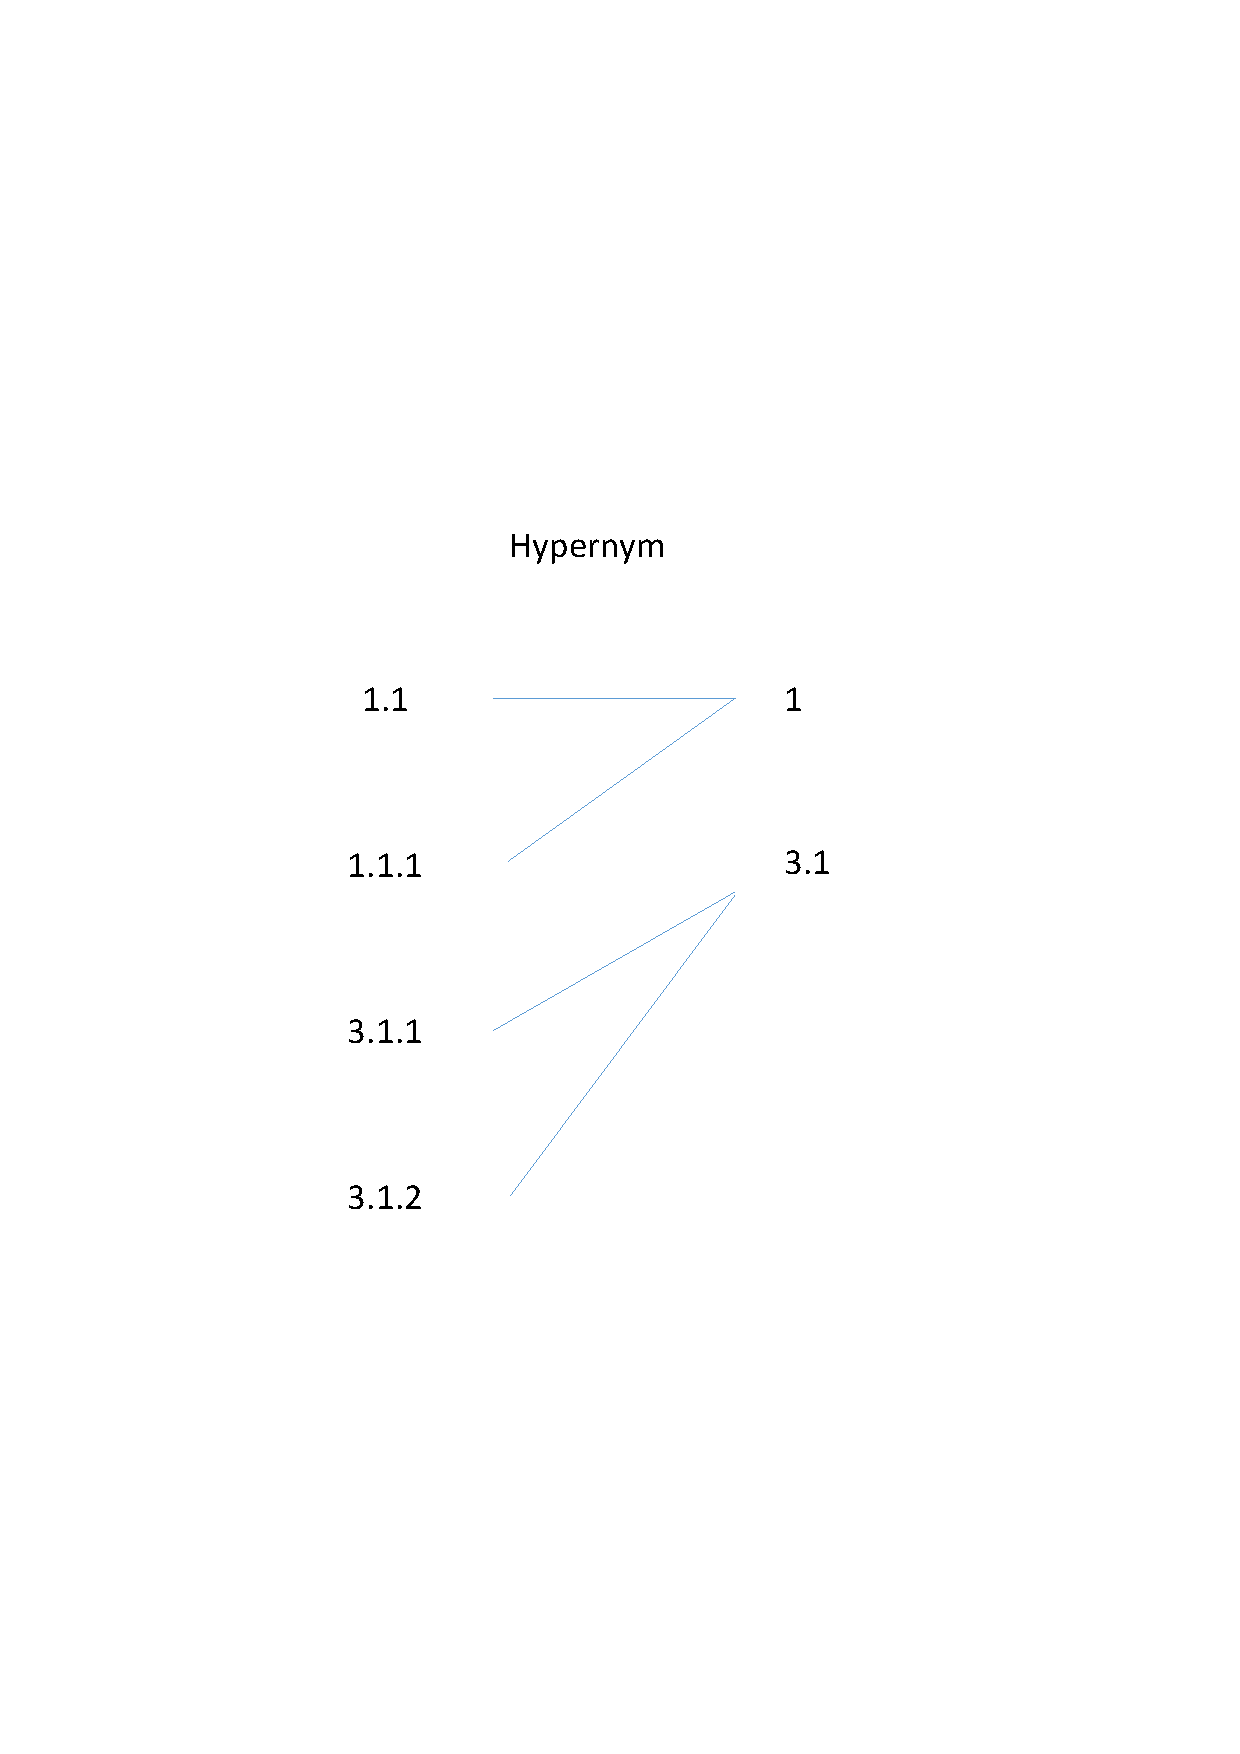
\includegraphics[scale=0.4]{figures/labeljoins}
% \caption{Join inverted lists}
%\label{fig:invertedlist}
%\end{figure}

The worst case complexity is $O(N^2)$, because the algorithm may compute each pair of strings with the prefix $p$. But this algorithm will skip many pairs of string for comparison. A theoretical analysis based on a random string model show that the average complexity is $O(\frac{N^2}{S^{\lfloor (1-\theta) \cdot l \rfloor}})$, where $N$ is the total number of elements in each list and $S$ is the maximal width of the taxonomy.




\begin{figure}[t]
\centering
\includegraphics[width=0.35\textwidth]{figures/prefixTrees}
 \caption{An example of TS join based on prefix trees (a circle means an internal element, but a rectangle means a real element)}
\label{fig:taxonomyexample}
\end{figure}



\begin{algorithm}
{\bf Input}: two collections of taxonomy nodes $S_1$ and $S_2$,  a threshold $\theta$ \\
{\bf Output}: string pairs $(s_1,s_2) \in S_1 \times S_2$, s.t. $TS(s_1, s_2) > \theta$
\begin{compactenum}[(1)]
\item Let $T_s$ and $T_t$ denote two compact tries for $S$ and $T$ respectively. 
\item Initialize two cursors in two tries.
\item {\bf WHILE} $\neg end(T_s) \wedge  \neg end(T_t)$ {\bf DO}
\item  ~~ $min$ = $\arg\min_{i}$($cur(C_i^1)$); $max$ = $\arg\max_{i}$($cur(C_i^1)$)
\item  ~~ {\bf IF} (possibleMatch(cur($T_{min}$),cur($T_{max}$))) {\bf THEN}
\item ~~ ~~ {\bf  IF} ($T_{min}$ is a real element)   {\bf THEN} Find(cur($T_{min})$,cur($T_{max}$))
 \item ~~~~ advance($T_{min}$)
 \item ~~ {\bf ELSE} Jump($T_{min}$)
 \item ~~ advance($T_{min}$)
\end{compactenum}
\smallskip
\textbf{Function} possibleMatch($s_1$,$s_2$)
\begin{compactenum}[(1)]
\item  $x = LCP(s_1,s_2)$
\item {\bf IF}  $(x > \theta \cdot min (s_1, s_2 )$  {\bf THEN} RETURN TRUE
\item   ~~ {\bf ELSE} FALSE
\end{compactenum}
\smallskip
\textbf{Procedure} Jump($T$)
\begin{compactenum}[(1)]
\item  read the next element that is not a descendant with the depth-first traversal
\end{compactenum}
\smallskip
\textbf{Procedure} Find($s_1$,$s_2$)
\begin{compactenum}[(1)]
\item  $x = LCP(s_1,s_2) $
\item {\bf IF} ( $|s_2| < max(\frac{x}{\theta},|s|)$) {\bf THEN}
\item ~~~~ {\bf FOR EACH} $i$=$|s_2|$ to $ \lceil max(\frac{x}{\theta},|s|) \rceil -1 $ {\bf DO}
\item ~~~~~~~ Add all real nodes under $s_2$ with the length $i$ to R;
\end{compactenum}
\caption{String joins with compact tries}
\label{alg:compactTrieJoin}
\end{algorithm}

\begin{theorem} Given two collections of nodes and a threshold $theta$, Algorithm \ref{alg:generaljoin} correctly finds all pair $n_1$ and $n_2$ such that $TS(n_1,n_2) > \theta$.
\end{theorem}


\begin{lem} Given two labels $s$ and $t$,  assume that $LCP(s,t) = x$. without the loss of generality, assume that $s<t$ by the lexicographical order, $TS(s,t) > \theta$ if and only if  $ x > \theta |s| $ and $  |t| < max(\frac{x}{\theta},|s|)$.
\end{lem}
\begin{proof}  $TS(s,t) > \theta$ $\Leftrightarrow$ $\frac{x}{|s|+|t|-x} > \theta \Leftrightarrow |t| < (\frac{1}{\theta}+1)x-|s|$. In addition, note that $|t| \geq x$. Then $x < (\frac{1}{\theta}+1)x-|s|$ $\Rightarrow$ $x > \theta |s| $, which concludes the proof.
\end{proof}


\smallskip
\smallskip

\begin{example}
Consider the example in Figure \ref{fig:taxonomyexample}, $\theta$=0.4. First, the cursors point to 2 and 2. possibleMatch return true. But 2 is not the real elements.  Then advance. Now $s_1$ =2.1 in $T_1$  and $s_2$=2.1.1 in $T_2$. Both real nodes. $x$=2.1, ($\frac{1}{\theta}+1)|x|-|s_1|$ = $5 > 3$. Therefore, (2.1, 2.1.1) and (2.1, 2.1.1.2) are added to the result pairs. Then the cursor advances, when $s_1$ =2.1.1.1, the result pair (2.1.1.1, 2.1.1.2) are added. Subsequently, the other two pairs (3.1, 3.1.1.1) and (3.2, 3.2.1.1) are added.
\end{example}

\smallskip
\smallskip

We next show the optimality: Given two compact tries, Algorithm \ref{alg:generaljoin} takes each node and find the  matching node with the trie operations. Therefore, each accessed pair $C_1$ and $C_2$ belong to the final results. Since the operation of output Line is equal to the size of the final results: we have the following optimality result:

\begin{theorem}   The computing cost of Algorithm \ref{alg:generaljoin} is linear to the sum of the size of the input and output.
\end{theorem}




